\documentclass{article}
\usepackage{graphicx}
\usepackage[margin=1.5cm]{geometry}
\usepackage{amsmath}

\begin{document}

\title{Friction Lab with Inclined Planes: Testing Friction dependence on Normal Force}
\author{Prof. Jordan C. Hanson}

\maketitle

\begin{figure}[ht]
\centering
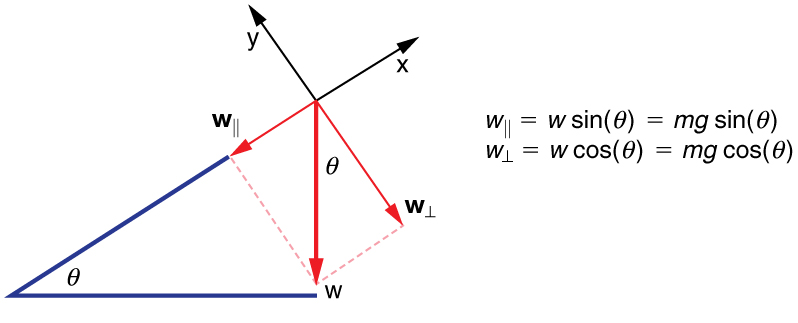
\includegraphics[width=0.75\textwidth]{incline.jpeg}
\caption{\label{fig:incline} The weight vector may be broken into two components: parallel and perpendicular.}
\end{figure}

\section{Introduction}

Recall that the static friction force is given by

\begin{equation}
f \leq \mu_{\rm s} N
\end{equation}

$N$ represents the normal force.  On a flat solid surface, $N = mg$.  On an inclined surface with angle $\theta$, the normal force balances the component of the weight vector perpendicular to the surface: $N = w_{\perp} = mg \cos\theta$.  The component of the weight vector parallel to the incline is $w_{||} = mg \sin\theta$.  The component $w_{||}$ can be balanced by friction if an object is on an inclined plane but not sliding.

Equate the static friction force $\mu_{\rm s} N = mg\sin\theta$ with $w_{||}$ to show that

\begin{equation}
\mu_{\rm s} = \tan\theta
\end{equation}

\section{Setup}

You will need the following objects: an index card, a small circular weight, and a protractor.  Place the weight on the index card and tilt the card upwards. The weight should remain in place.  Use the protractor to measure the angle \textit{at which} the weight just begins to slide.

\section{Data Collection}

Using three different masses $m_1$, $m_2$, and $m_3$, fill in Tab. \ref{tab:meas} on the next page with measurements of $\theta$ in degrees.  Take three measurements for each mass and list them in trials 1, 2, and 3. \\ \vspace{2cm}

\begin{table}
\centering
\begin{tabular}{| c | c | c |}
\hline
Mass (grams) & Angle (degrees) & Trial \\ \hline
& & 1 \\ \hline
& & 2 \\ \hline
& & 3 \\ \hline
& & 1 \\ \hline
& & 2 \\ \hline
& & 3 \\ \hline
& & 1 \\ \hline
& & 2 \\ \hline
& & 3 \\ \hline
\end{tabular}
\caption{\label{tab:meas} List the mass in grams in the first column, and keep the same mass for three trials.  Record the angle in degrees.}
\end{table}

Convert your angles in Tab. \ref{tab:meas} to $\mu_{\rm s}$-values.  Produce an average and standard deviation below: \\ \vspace{1cm}

$\mu_{\rm s} = \underline{~~~~~}\pm\underline{~~~~~}$ \\ \vspace{0.5cm}

Share your result with the instructor to build the class-wide table of results.

\end{document}
